Generating data as if it was derived from a CNL model is not straight forward because of the complicated correlations across alternatives and nests. We employ a shortcut which allows us to sample sequential multinomial trials and convert these into proper nested and cross-nested trials using sampling based on the probabilities derived above. As an example notice in \eqref{eq: likelihoodprob} that the last term $\frac{\alpha_{im}z_i^{\mu_m}}{\sum_j \alpha_{jm} z_j^{\mu_m}}$ is essentially the ordinary multinomial choice probability with a bit of added complexity in the form of $\alpha$'s and $\mu$'s, and that for a child-node with only one parent-node the first term will provide only one hit in the numerator as all other $\alpha_{jm}$ are $0$. Similarly the denominator will produce one hit for each value of $m$. In the case of two nested binary outcome choices, \eqref{eq: likelihoodprob} thus collapses to the product of the probabilities of two individual multinomial trials weighted by $\mu_m$'s. This pattern extends nicely to larger nested structures, making it easy to generate datasets of the nested kind.
\\ \\
In the cross nested model there's the added difficulty of partial node-membership, that is $\alpha_{im} \neq \{0,1\}$ in general. Our approach handles this simply by drawing from the probability density $\textrm{Pr}(\mathcal{J} = i |m)$ as derived above. In this way we simulate full paths through the tree, with each step modelled as a logit-like trial, now indcluding $\alpha$ parameters. In this way we get one choice per individual per nest. This gives us one to many choices as we observe a choice $(c_1|c_2)$ at $n_1$ and a choice $(c_2|c_3)$ at $n_2$. Naturally these cannot co-occur, and thus we drop observations according to the individuals choice at $R$. Appendix \ref{app: vectorization} contains a discussion of the computational issues this double counting gives.

\subsection{DGP structure in simulated data}
For the sake of simplicity we restrict out estimator testing to datasets with simple nesting structures. We construct both a dataset of nested and cross-nested data, each with three observed outcomes $c_1, c_2, c_3$. A visual impression of the DGP's is given in figure \fref{fig: simpletree}. In the nested case we create two nests $m_0$ and $m_1$ each with binary outcomes, and linked by one option in $m_0$ to the root of $m_1$. To accommodate cross-nesting we have to add a third nest, making both of the roots child-nodes $n_1,n_2$ unobserved.

\begin{figure}[!h]
  \begin{center}
  \def\svgwidth{0.90\columnwidth}
  \import{03_figures/}{simpletrees.pdf_tex}
  \end{center}
  \caption{The nesting structures employed as simulated data.}
  \label{fig: simpletree}
\end{figure}

This kind of cross nesting is indeed very simple compared to the capabilites of CNL, but are computationally less demanding while maintaining the important trait that choosing branch ($n_1$ or $n_2$) does not restrict the choice-set to proper sub-branches.
\\ \\
As the data is multinomial one need to specify a vector of $\beta$-parameters associated with each choice in the dataset excluding the root node $R$. In doing so researchers might choose to include different variables at different nodes. To maximize the amount of information gained from each observation we choose not to do this, and instead include the two independent vectors $x_1, x_2$ as regressors in all utility equations. Since there are five choices in the CNL DGP, we get a total of 5 equations (4 in the NL case) of the form
\begin{equation}
V_j = [x_1 \ x_2] \beta_j
\end{equation}

\begin{figure}[h]
  \begin{center}
  \begin{subfigure}{0.45\linewidth}
    \caption{NL}
    \centering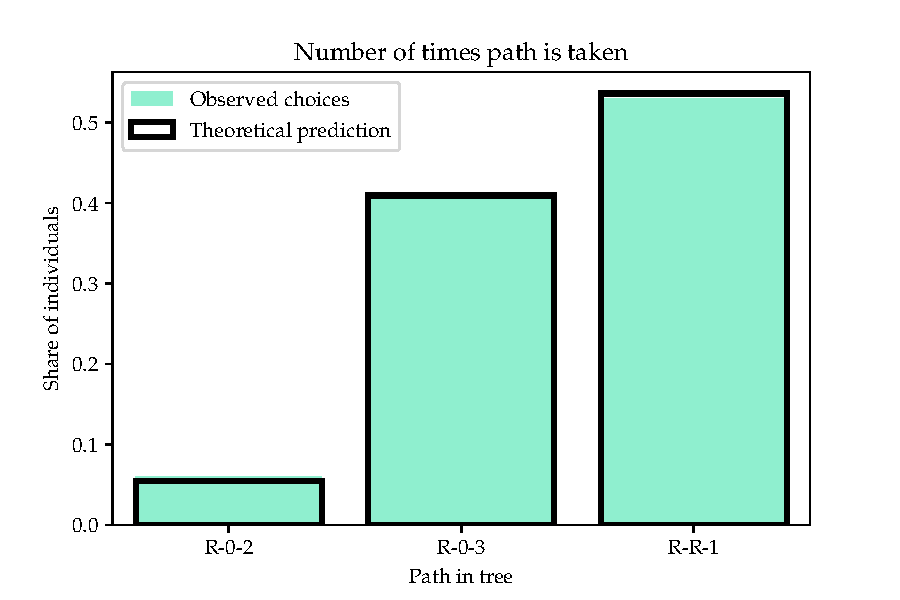
\includegraphics[width=\linewidth]{03_figures/choice_fractions_NL.pdf}
  \end{subfigure}
  \begin{subfigure}{0.45\linewidth}
    \caption{CNL}
    \centering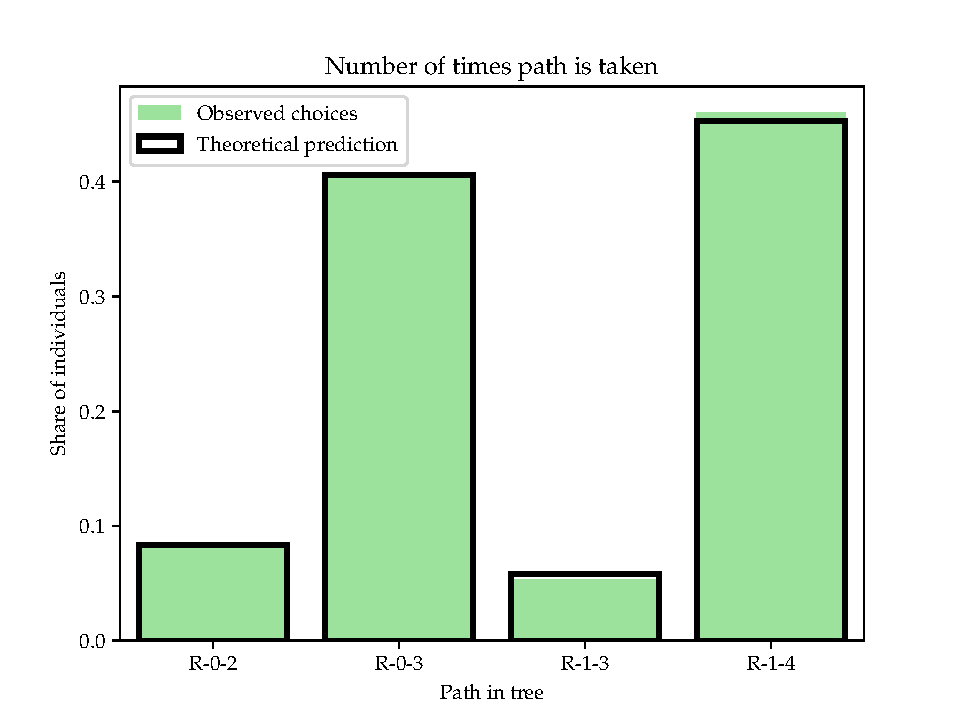
\includegraphics[width=\linewidth]{03_figures/choice_fractions.pdf}
  \end{subfigure}
  \caption[Actual and theoretical choice probabilities.]{Actual and theoretical choice probabilities. The x-axis is read as follows. From left to right is the path through the tree, with $R$ being the root, and apart from that the mapping is $(n_1, n_2, c_1,c_2,c_3) \rightarrow (0,1,2,3,4)$.}
  \label{fig: choiceprobs}
\end{center}
\end{figure}

By simulating and selecting data as described above we construct a dataset of 100 "individuals", and their hypothetical decision at every node of the CNL tree depicted in figure \ref{fig: simpletree}. The expected probability of a given path (i.e. $R\rightarrow n_1 \rightarrow c_2$) is then given by the product of nest-conditional probabilities at each step, and we can quite easily calculate these. Since we simulate the entire structure and not just the lowest nodes, we can trace out otherwise un-separable paths in the tree. Figure \ref{fig: choiceprobs} shows the observed share of choosers following a given path in the CNL tree and compares it to the theoretical number. First of all, the apparent dissymmetry of the CNL path shares compared to the ones in the NL model is useful in understanding the flexibility of the CNL model. Secondly this figure serves as a way of validating that our code functions as anticipated.


\subsection{Data validation}
We use a number of tests to ensure the DGP is correctly implemented. These all rely on the various probabilities debated in the section on estimation. Specifically we know that the following identities must hold true
\begin{equation}
  \begin{split}
  &\sum_{i\in \mathcal{C}} \textrm{Pr}(i|\mathcal{C}) = 1 \\
  &\sum_{m\in \mathcal{M}} \textrm{Pr}(m|\mathcal{C}) = 1
  \end{split}
\end{equation}
And finally we also know $\forall m : \ \sum_{i \in m} \textrm{Pr}(\mathcal{J} = i | m) = 1$. That is 1) the summed probability of making choice $i$ over the entire choice set must be 1, 2) the summed probability of entering nest $m$ summed over all nests must be 1 and 3) Within all nests, the summed probability of choosing $i\in m$ must be 1 when conditioning on being in the specific nest.
\\ \\
Knowing that our code passes all of these criteria we are confident that we simulate data from the correct DGP.

\subsection{Real data (the DREAM dataset)} \label{subsec: dreamdata}
In order to model probabilities regarding the course of those that are out of the labour market on sick leave, we use weekly data from the semi-governmental institution \textit{The Danish Institute for Economic Modelling and Forecasting}, the DREAM Group, based on their agreement with LO, The Danish Confederation of Trade Unions. More specifically the december 2017-version of the microeconometric database covering week-by-week socioeconomic status of all 5,6 million Danish citizens subdivided into 36 labour market categories. The registry lays the foundation for their socioeconomic projection model \citep{dream_danish_2018}. Table \ref{tab:sumstats} show summary statistics for the sample.

For simplicity we model the one-year course for the group of 84.123 persons on sick leave that received unemployment benefits ("sygedagpenge") in week 48 of 2016 (last week of november). Thus, the selection besides from being those hit by prolonged illness is limitied to those that have been a member of an unemployment insurance fund and have been in work recently in order to fulfill the conditions for receiving unemployment benefits.

\begin{table}
  \centering
\begin{tabular}{lrrr}
\toprule
{} &         $c_1$ &         $c_2$ &         $c_3$ \\
\midrule
All       &  0.12 &  0.35 &  0.53 \\
Male      &  0.11 &  0.34 &  0.55 \\
AC        &  0.11 &  0.27 &  0.62 \\
Age 15-30 &  0.14 &  0.26 &  0.60 \\
Age 30-40 &  0.13 &  0.32 &  0.55 \\
Age 40-50 &  0.11 &  0.35 &  0.54 \\
Age 50-60 &  0.11 &  0.40 &  0.49 \\
\bottomrule
\end{tabular}
\caption{Summary statistics: distribution of choices for subgroups in data.}
\label{tab:sumstats}
\end{table}

Our dataset is then reduced to 73.864 individuals by dropping the 10.259 above 60 years olds ultimo november 2017 in order to avoid interference with ordinary retirement schemes. Furthermore 6.348 are dropped who in week 48 of 2017 (last week of november) where on either paternity leave, no longer living in Denmark, dead, or neither employed nor receiving unemployment benefits (i.e. no information on one's livelihood).
\\ \\
We end up with 67.516 observations for which the following regressors are included:
  \begin{equation} \label{eq: DREAM_regressors}
    x = \left[\textrm{male, ac, age, age}^2\right]
  \end{equation}
Where \textit{ac} is a dummy for the 7 pct. of individuals in the dataset who are members of one of the four unemployment insurance funds for college graduates (\textit{AJKS}, \textit{AKA}, \textit{CA} or \textit{MA}).
\\ \\
The choices are defined based on their socioeconomic status in week 48 in 2017 (one year after having been on sick leave).
  \begin{itemize}
    \item[$c_1$] (\textit{"Ordinary unemployment"}): Receiving unemployment benefits while actively seeking jobs.
    \item[$c_2$] (\textit{"Sick"}): On sick leave ("sygedagpenge"), early retirement due to sickness ("førtidspension"), subsidized work on reduced hours due to sickness ("fleksjob"), or being in one of several courses for partially sick where one's amount of work-ability is examined.
    \item[$c_3$] Ordinary employment or under education.
  \end{itemize}
As the linear RUM setup (equation \ref{eq: utility_general}) is based on utility maximizing agents, our estimation model is to assume that the choice between $c_1$ and $c_3$ depends on the opportunity cost of being out of labour, i.e. as men and college graduates in general earn above the median wage we use these dummies as proxies for having a higher utility from choosing $c_3$ relative to $c_1$, besides from the other characteristics associated with ticking theese boxes which also for the most part drag in the direction of $c_3$. As a higher age is also correlated with a higher wage we similarly can expect older people to have a higher probability of choosing $c_3$ while a squared term for age allows for nonlinearity such that there could exist a maximum point for age from which on the probability of choosing $c_3$ over $c_1$ could be decreasing instead. Leaving the world of utility maximizing individuals for a second, the employer's side of an imperfect labour market might also have preferences regarding an employer's ideal age that can be described by a similar 2nd order polynomial which would further increase the effect. Given expectations about different probabilities for $c_1$ and $c_3$ based on regressors we assume that the error terms tend towards being uncorrelated and that there should not exist cross-nesting between this pair of alternatives.

$c_2$ on the other hand is difficult to fit into the RUM-setup. Thus we assume that being too sick to be available for the ordinary labour market is mainly correlated with a higher age while correlation with the other regressors is less significant. Assuming a near random draw of those hit by a more permanent sickness, we expect the hidden attributes in the error term to be both correlated with both those who choose $c_1$ and $c_3$ and thus we allow for cross-nesting with both nest $n_1$ and $n_2$, see the CNL-structure in \ref{fig: simpletree} above.
